\documentclass[11]{article}
\usepackage[utf8]{inputenc}

\usepackage{cite}

\usepackage{float}
\usepackage{graphicx}
\usepackage{subcaption}
\author{Xavier Martín Ballesteros and Adrià Cabeza Sant'Anna \\ \small UNIVERSITAT POLITÈCNICA DE CATALUNYA}
\title{Flower detection using features\\ \large{Computer Vision, UPC}}
\date{\today}

\begin{document}
\maketitle
\vspace*{\fill}

\includegraphics[scale=0.4]{UPClogo.png}\par\vspace{1cm}

\newpage
\tableofcontents
\newpage 

\section{Introduction}
The aim of this assignment is to classify 12 different types of flowers using feature extraction. 

We have first implemented several ways to extract features that we believed could be key in order to classify correctly the flowers, we tested them, and using different classifiers (decisions trees, SVM or random forest) have tested the accuracy, specificity or sensitivity. 

\section{Descriptors}
In the following sections we will introduce different descriptors we have used to find those valuable features.

\subsection{Compactness}
\subsection{Color Histogram}

\begin{figure}[H]
	\centering
	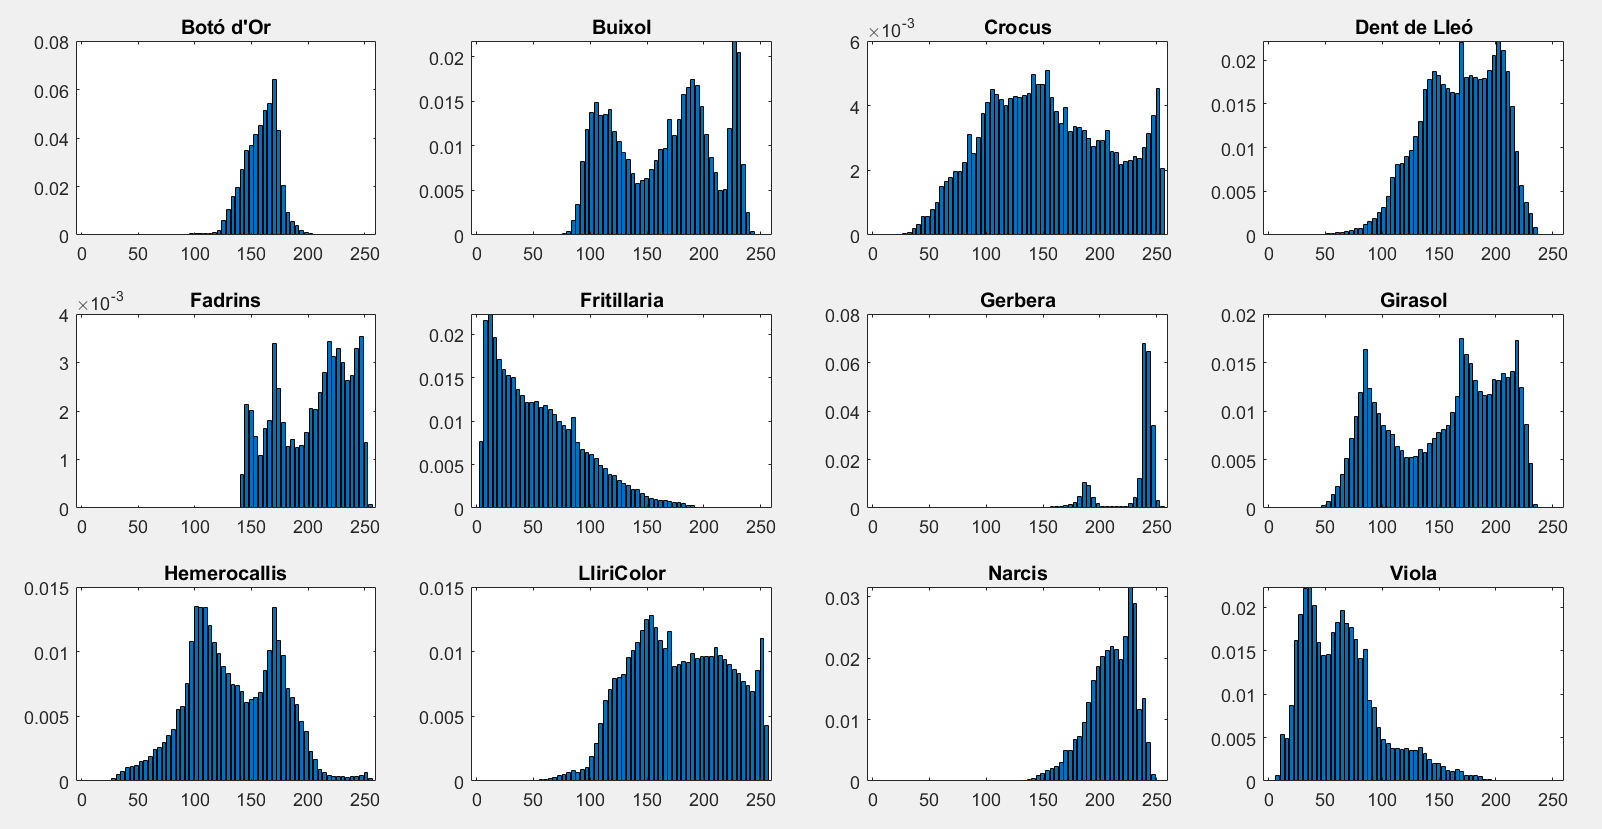
\includegraphics[scale=0.35]{images/colorHistogram1}
	\caption{Prova1.}
\end{figure}

\begin{figure}[H]
	\centering
	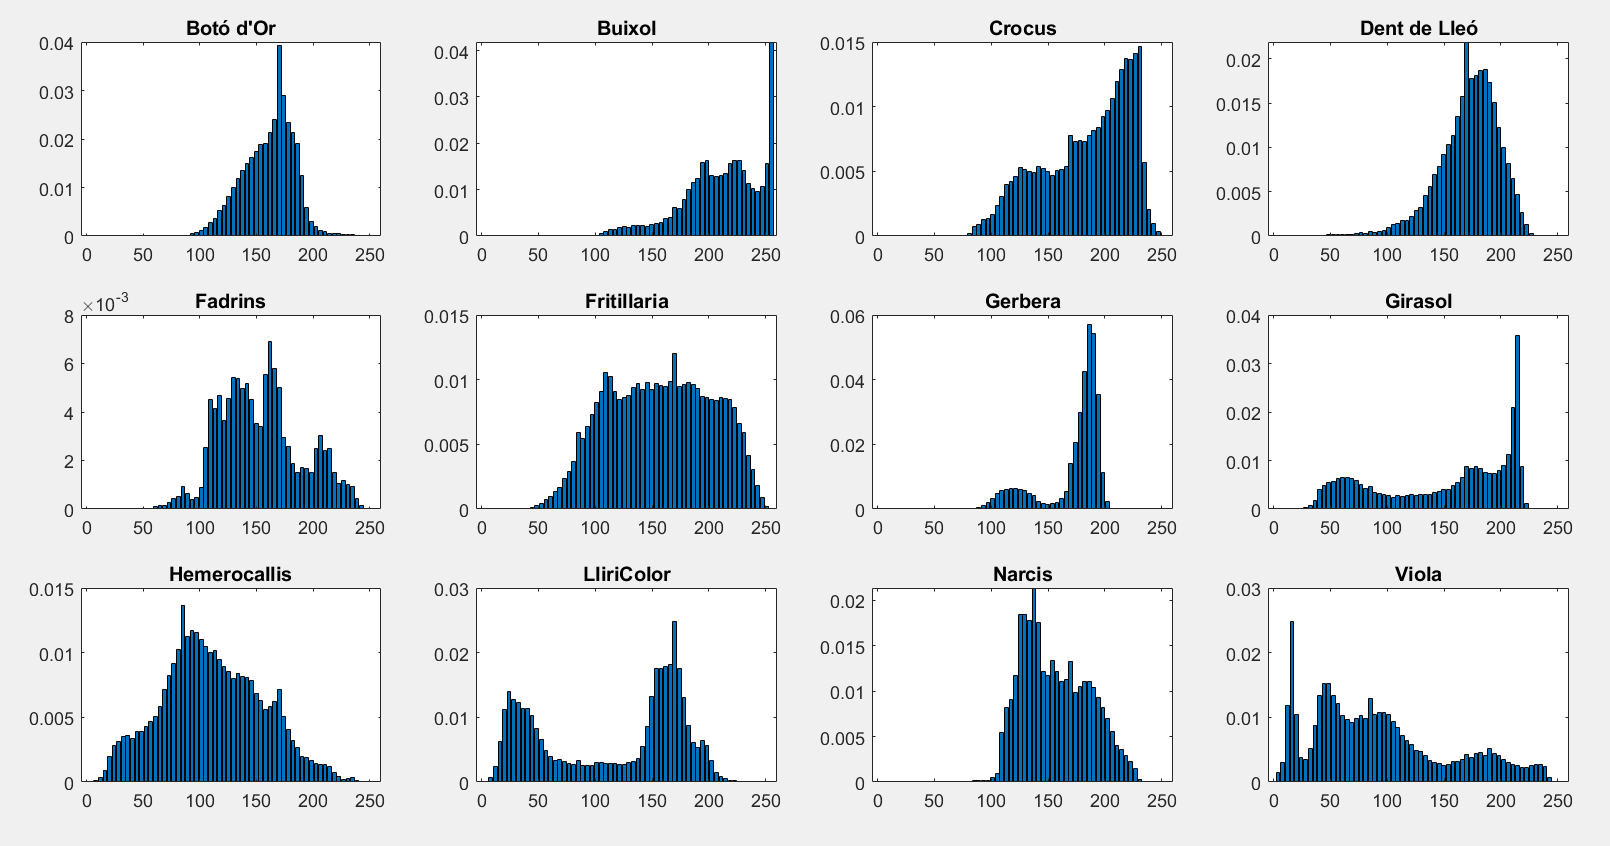
\includegraphics[scale=0.35]{images/colorHistogram2}
	\caption{Prova2.}
\end{figure}

\begin{figure}[H]
	\centering
	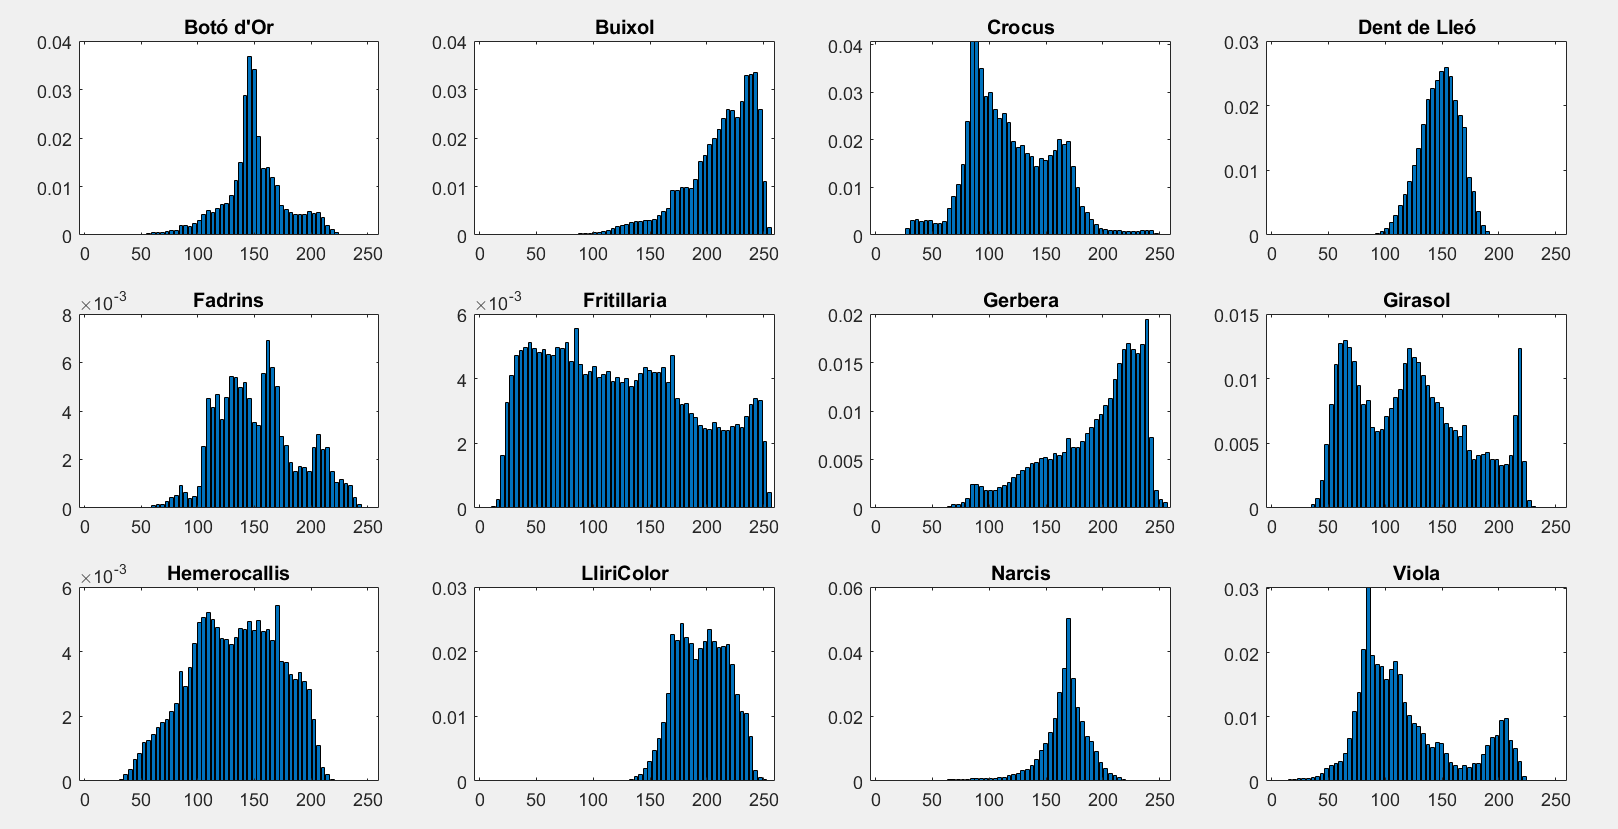
\includegraphics[scale=0.35]{images/colorHistogram3}
	\caption{Prova3.}
\end{figure}

\subsection{Number of petals}

This descriptor was one of the most difficult to think of. It can be done in several ways so we first had to choose in which way we wanted to attack the problem. In our case we decided to skiz the flower.
\medskip

To do so we used \textit{bwmorph(image, 'skel', inf)} from Matlab. This	 creates the skeleton iterating as many times as necessary in order to not see any change between iterations (until it converges). Then we observed that sometimes the skiz did not touch the contourn of the flower so we could not really count the petals; to solve it we applied an small erosion. The value of the disk structure was chosen based on several trials. 
\medskip

\noindent In this example using \textit{Boto d'Or} we get as a result 5 petals:
\begin{figure}[H]
    \begin{subfigure}[t]{.49\linewidth}
    \centering
  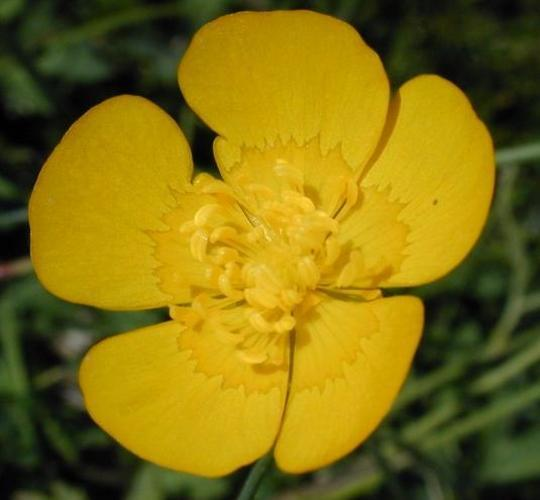
\includegraphics[scale=0.25]{images/numberOfPetalsOriginal.jpg}
  \caption{Original}
  \label{original}
    \end{subfigure}
    \begin{subfigure}[t]{.49\linewidth}
    \centering
    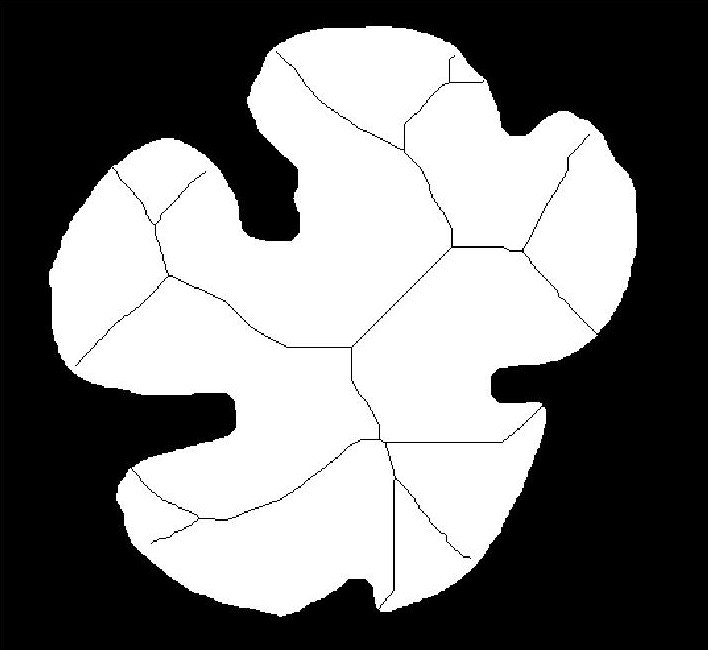
\includegraphics[scale=0.2]{images/numberOfPetals.jpg}
    \caption{Skez of the image}
    \label{skez}
    \end{subfigure}
\end{figure}


\subsection{Relative position of the centroid}

Just evaluating the position of the centroid would have been useless, it is not a feature of the flower per se. It can vary depending on the angle of the photo or the distance. However, if we calculate the relative position we can get really powerful information. 
\\

This two flowers, for example, should have really different values for this descriptor and it could be key in order to differenciate them in our classifier:
\begin{figure}[H]
    \begin{subfigure}[t]{0.45\textwidth}
    \centering
  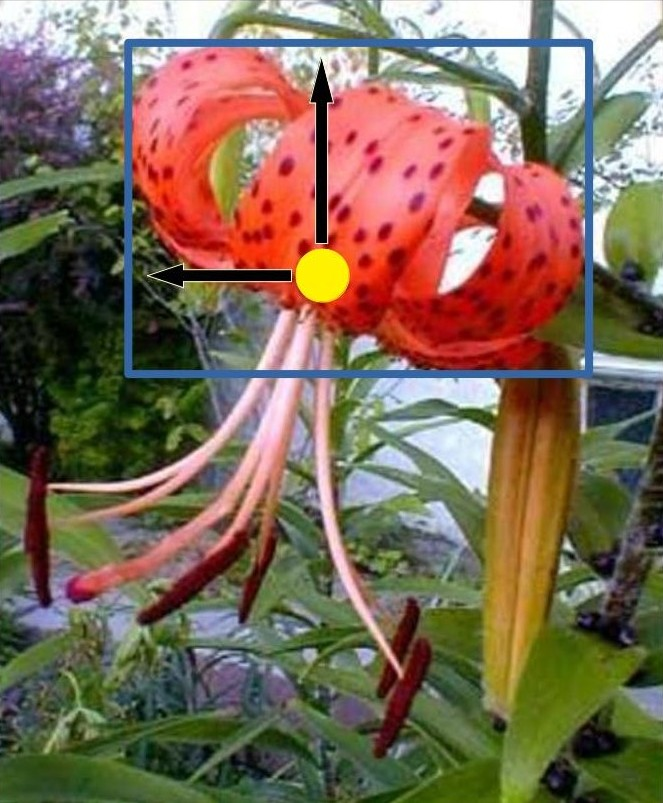
\includegraphics[scale=0.2]{images/hemerocallisCentroid.jpg}
    \caption{Centroid and bounding box of a \textit{Hemerocallis}}
    \label{centroidHemerocallis}
    \end{subfigure}
    \begin{subfigure}[t]{0.45\textwidth}
    \centering
    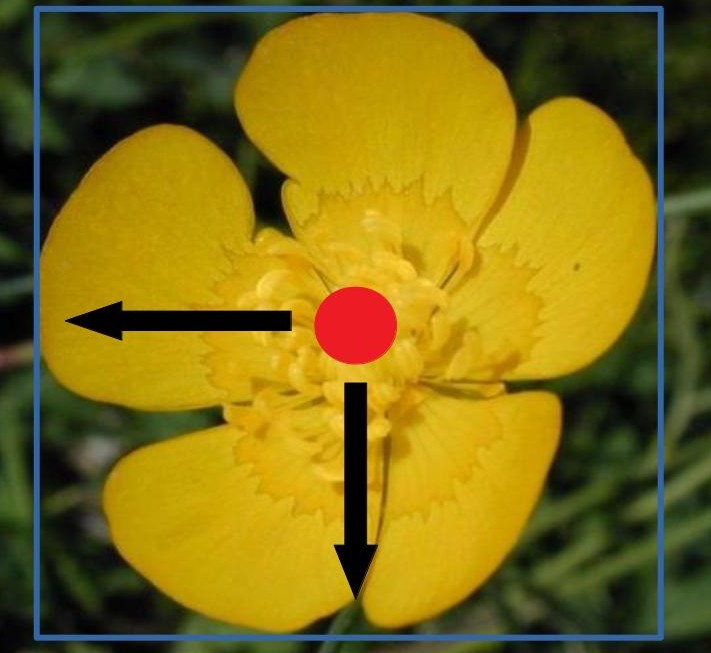
\includegraphics[scale=0.2]{images/GirasolCentroid.jpg}
    \caption{Centroid and bounding box of a \textit{Girasol}}
    \label{centroidgirasol}
    \end{subfigure}
\end{figure}

The way our descriptor is implemented is the following: we get the first and last pixels of X and Y axis in order to create the \textbf{bounding box}, then using regions props we get the \textbf{centroid of the flower} and finally we calculate the \textbf{relative position} of the centroid over the bounding box. 
\medskip

In this example using \textit{TBD} we get as a result X Y: 

\begin{figure}[H]
	\centering
	\includegraphics[scale=0.45]{images/DUNNO}
	\caption{Centroid and bounding box output of a \textit{TBD}}
	\label{centroidTBD}
\end{figure}



\subsection{Hoggs form: Orientation}
Available at the \textit{Matlab Computer Vision Toolbox}
\subsection{Fourier descriptor: Shape}


\section{Classifier}



\section{Data augmentation}
In order \textbf{to strenghten our descriptors} we have also used the following public repository:  \textit{Albumentation: fast image augmentation library and easy to use wrapper around other libraries}(see more in References), which proporcionates facilities to augment the dataset including several transformations like: flipping, blurrring, RGB Shifting, Random contrast, Random brightness, etc...
\medskip

To decide which transformations we wanted to apply, we looked first to our descriptors and the importance of each feature. For example, we discarted the Channel Shuffle because we believe that the color is very important for our implementation. Then, based on trial and error, we picked some of them which gave us an overall better result. Finally we are using random variations of:
\begin{itemize}
    \item Brightness and Contrast
    \item Blur
    \item Rotations
    \item Flips
\end{itemize}
For example let's suppose that we are working with this \textit{Boto d'Or} image:
\begin{figure}[H]
    \centering
    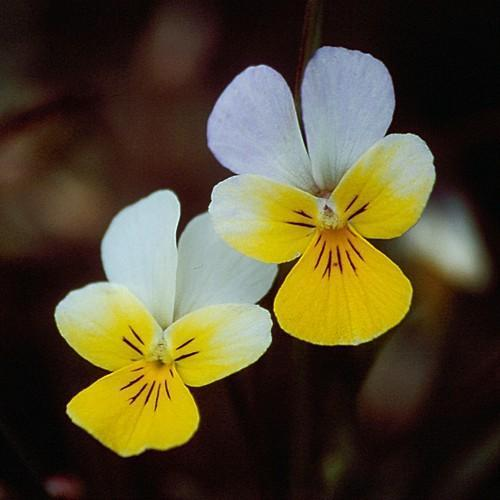
\includegraphics[scale=0.2]{images/original.jpg}
    \caption{Original picture}
    \label{original}
\end{figure}

The script we have implemented would apply the following transformations: 

\begin{figure}[H]
    \begin{subfigure}[t]{0.45\textwidth}
    \centering
  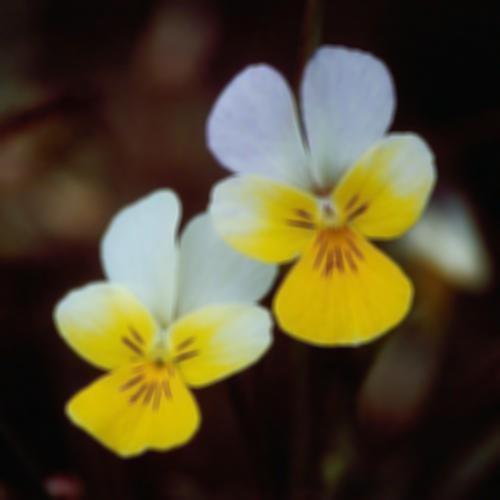
\includegraphics[scale=0.2]{images/blur.jpg}
    \caption{Blur transformation}
    \label{blur}
    \end{subfigure}
    \begin{subfigure}[t]{0.45\textwidth}
    \centering
    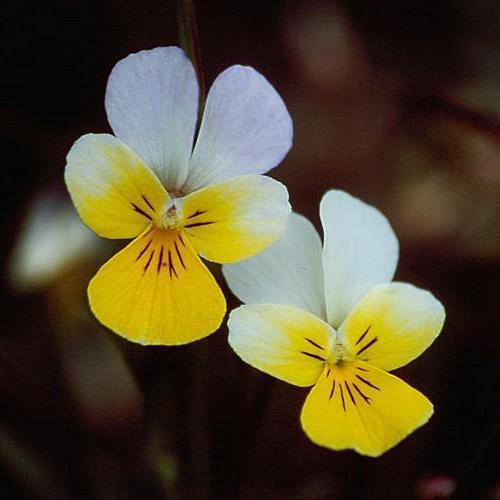
\includegraphics[scale=0.2]{images/horizontal.jpg}
    \caption{Horizontal Flip transformation}
    \label{horizontalflip}
    \end{subfigure}
\end{figure}

\begin{figure}[H]
    \begin{subfigure}[t]{0.45\textwidth}
    \centering
  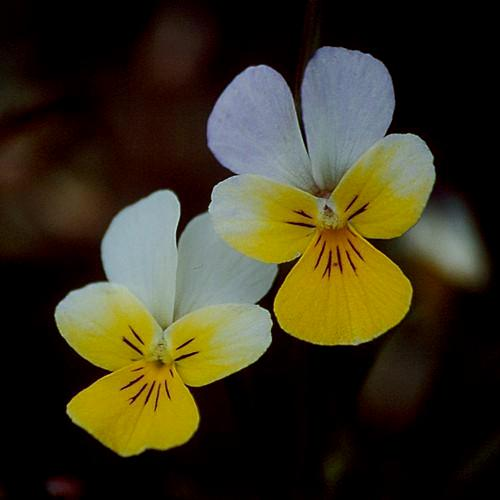
\includegraphics[scale=0.2]{images/brightness.jpg}
    \caption{Brightness and Contrast transformation}
    \label{brightness}
    \end{subfigure}
    \begin{subfigure}[t]{0.45\textwidth}
    \centering
    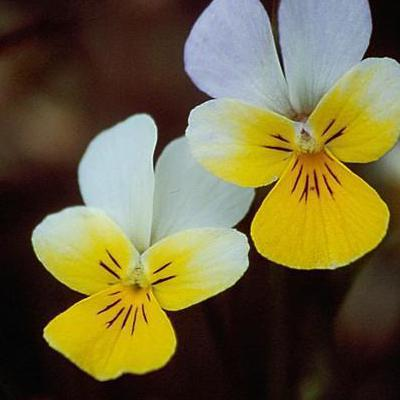
\includegraphics[scale=0.2]{images/scale.jpg}
    \caption{Scale transformation}
    \label{scale}
    \end{subfigure}
\end{figure}




\newpage
\begin{thebibliography}{100}

\bibitem{Albumentations}
    A. Buslaev (2018). Based on \textit{Albumentations: fast and flexible image augmentations} [online]. Paper available at:https://arxiv.org/abs/1809.06839. Code available at:https://github.com/albu/albumentations  [Accessed 3 June. 2019].

%%%%%%%%%%%%%%%%%%%%%%%%%%%%%%%%%%%%%%%%%%%%%%%%%%%%%%%%%%%%%%%%%%%%%%%%%%%%%%%%%%%%%%%
%\bibitem{Analysis of image Thresholding Methods for application to augmented reality enviornments}
%D. Martín Carabias (2012). \textit{Analysis of image Thresholding Methods for application to augmented reality enviornments.} [online] UCM. Available at: https://eprints.ucm.es/16932/1/Tesis\_Master\_Daniel\_Martin\_Carabias.pdf [Accessed 14 Mar. 2019].


%\bibitem{A survey of Thresholding Techniques}
%P. K. Sahoo, S. Soltani, K.C. Wong and Y.C. Chen (1988). \textit{A survey of Thresholding Techniques}. University of Waterloo, Waterloo, Canada  [Accessed 16 Mar. 2019].

%\bibitem{}N. Otsu, \textit{A Threshold Selection Method from Gray-Level Histograms}, in IEEE Transactions on Systems, Man, and Cybernetics, vol. 9, no. 1, pp. 62-66, Jan. 1979.
%[online] Available at http://ieeexplore.ieee.org/stamp/stamp.jsp?tp=\&arnumber=4310076\&is
%number=4310064 [Acessed 17 Mar. 2019].

%\bibitem{}Dr. Andrew Greensted (2010), \textit{Otsu Thresholding}. [online]. Available at http://www.labbookpages.co.uk/software/imgProc/otsuThreshold.html [Accessed 17 Mar. 2019].

%\bibitem{}Senthilkumaran,  N.  \&  Sivapriya,  M.  (2017),  \textit{Riddler's  Thresholding Algorithm  for  DNA  Image  Using  ISODATA  Modified  Algorithm} Journal  of Information Technology, Vol.3, No.2, pp.41-48. [online] Available at: http://www.ijitjournal.org/volume-3/issue-2/IJIT-V3I2P9.pdf [Accessed 17 Mar. 2019].

\end{thebibliography}

\end{document}
